O algoritmo responsável por efetuar o desvio de obstáculos recebe como
entrada um vetor indicando a direção e a velocidade a serem aplicadas
ao robô e as leituras do laser. Ele retorna um novo vetor
representando a direção e velocidade calculadas de modo que o robô
tenda a seguir na direção desejada, desviando de eventuais obstáculos.
O vetor de direção é representado por uma mensagem do tipo
\lcode{geometry\_msgs/Twist}. As leituras do laser são representadas
por mensagens do tipo \lcode{sensor\_msgs/LaserScan}. Um diagrama
contendo os nós e tópicos utilizados pelo sistema podem pode ser
observado na Figura \ref{fig:diag_proj_ros}.

\begin{figure}[H]
    \centering
    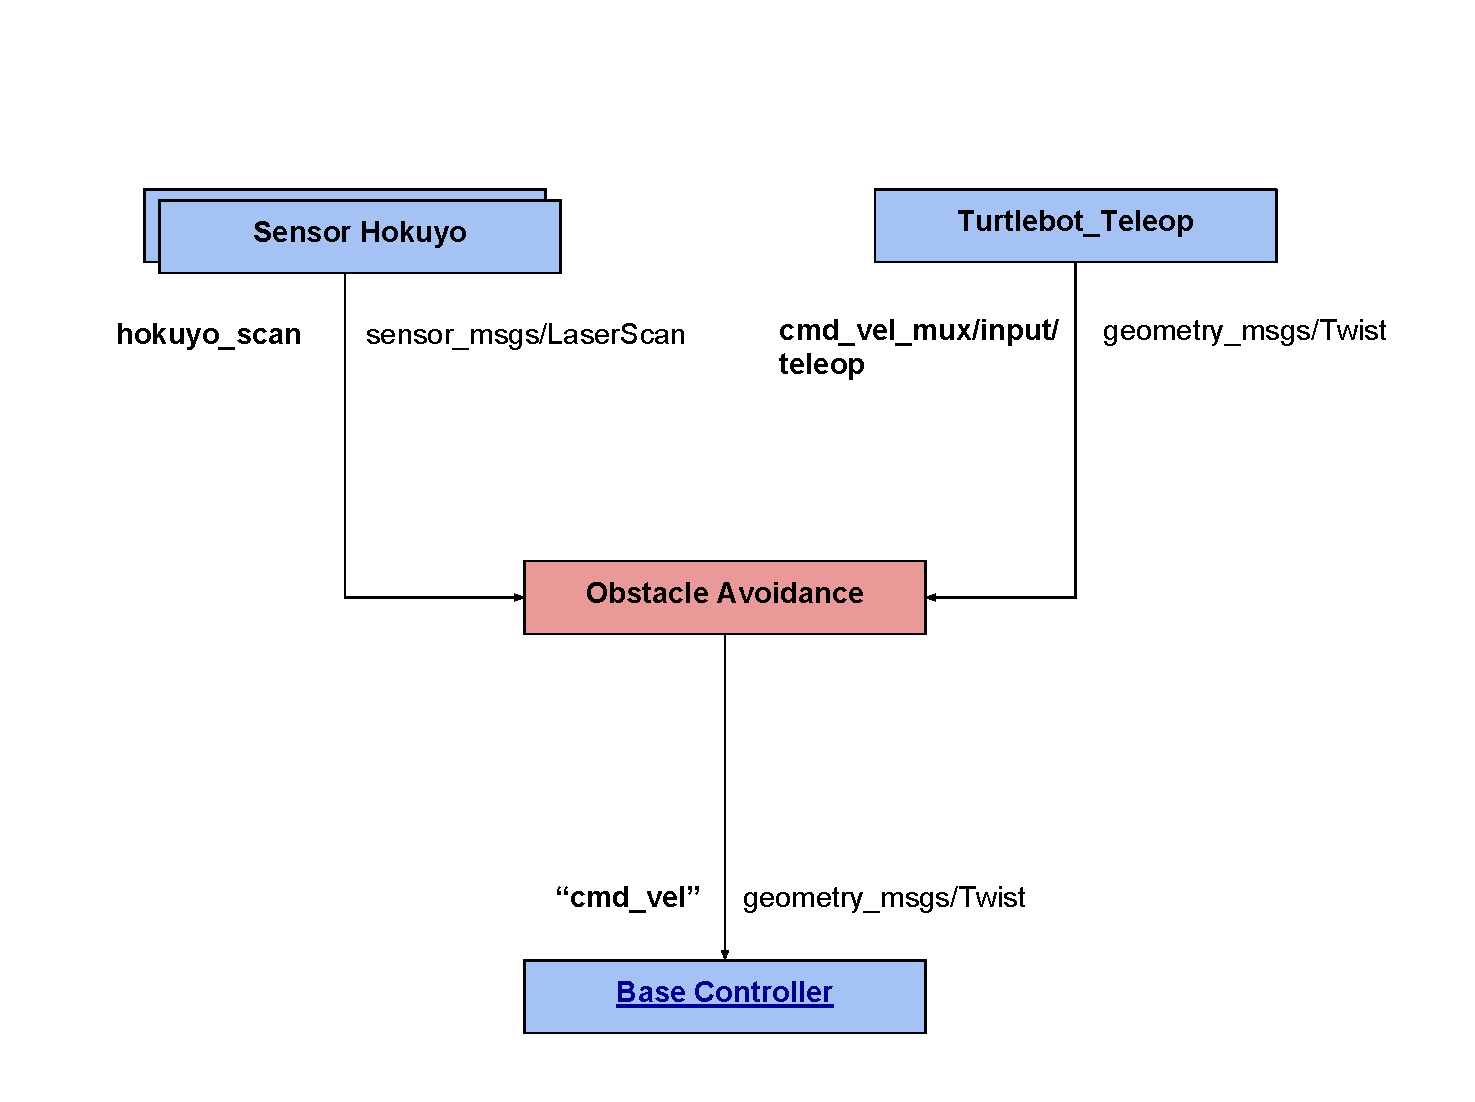
\includegraphics[width=0.85\textwidth]{img/Diagrama_Projeto_ROS.pdf}
    \caption{Diagrama de nós do sistema.}
    \label{fig:diag_proj_ros}
\end{figure}

O tópico \lcode{hokuyo\_scan} fornece as leituras do laser e o tópico
\lcode{cmd\_vel\_mux/input/} fornece os vetores indicando a direção que
o robô deve seguir. O módulo \textbf{Obstacle Avoidance} representa o
algoritmo de desvio de obstáculos, o qual posta os vetores resultantes
no tópico \lcode{cmd\_vel} do robô.

\subsection{Detecção de Obstáculos}

Foi utilizado um algoritmo implementando a técnica de Bubble Band  (Seção \ref{sec:bubbleband}). Caso alguma amostra do sensor aponte um valor
de distância menor que o limite da "bolha", é chamado o algoritmo VFH (Seção \ref{sec:vfh}). Como o
laser utilizado fornece, 40 vezes por segundo, aproximadamente 728 amostras de distâncias
(\textit{ranges}), decidiu-se verificar, a cada
dez amostras, a presença de obstáculos em uma extensão de $-90°$ a $+90°$ em relação
ao eixo central do robô (Figura \ref{fig:laser_scan}). O algoritmo de
detecção de obstáculos implementado pode ser observado no Código
\ref{cod:checkObstacles}.

\begin{figure}[H]
    \centering
    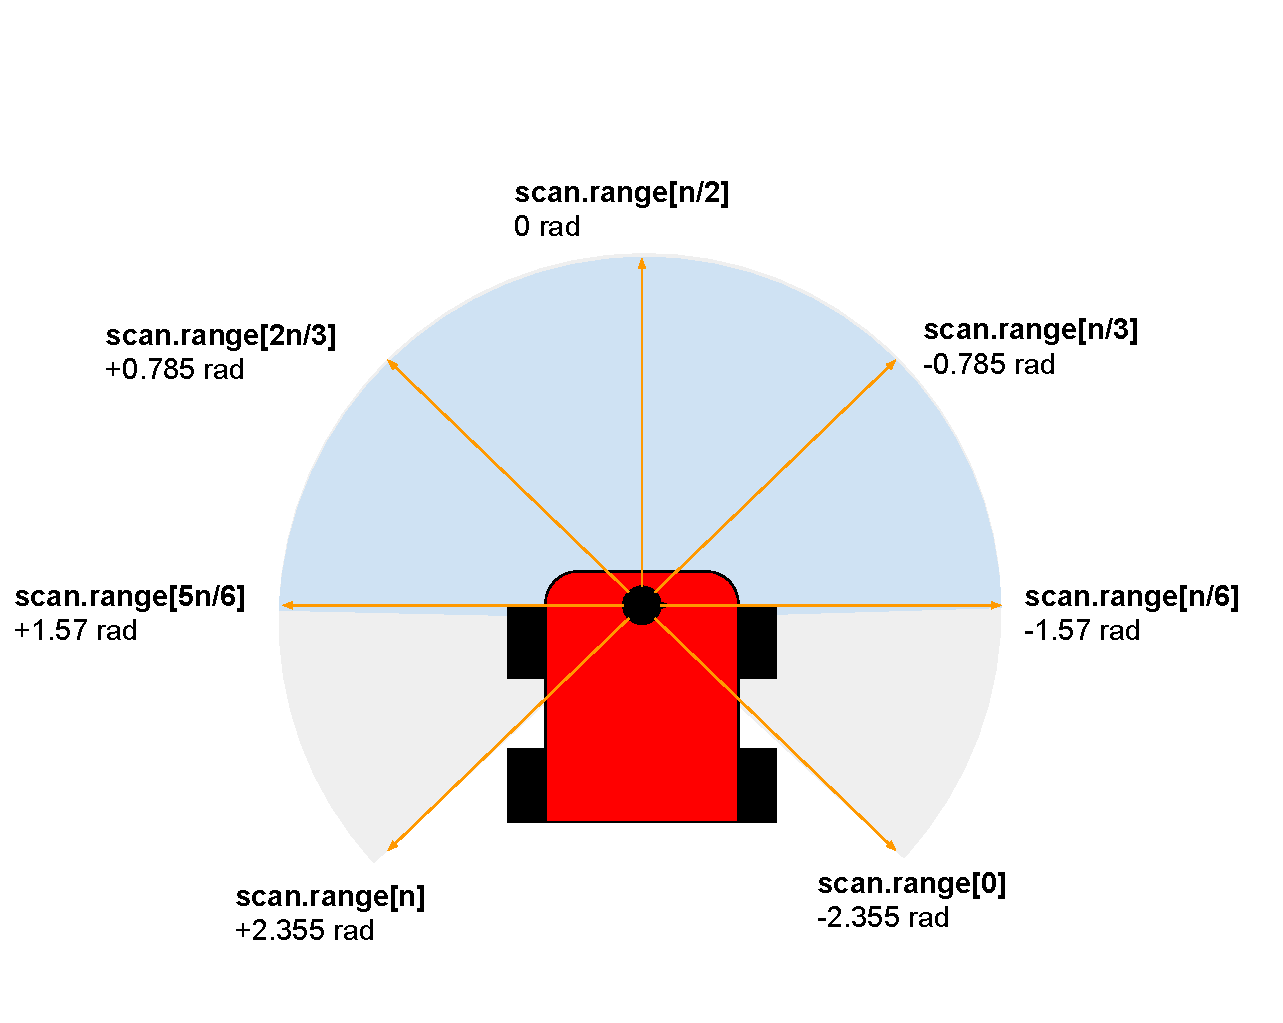
\includegraphics[width=0.85\textwidth]{img/SensorAngulos.pdf}
    \caption{Leitura do sensor laser.}
    \label{fig:laser_scan}
\end{figure}

\begin{lstlisting}[frame=single, label=cod:checkObstacles, style=customc,
caption={Algoritmo de Verificação de Obstáculos}]
bool checkForObstacles(sensor_msgs::LaserScan msg, float limite){
    
    int numero_amostras = (int) floor((msg.angle_max - msg.angle_min) / msg.angle_increment);
    
    //Le as amostras a cada 10 unidades
    for (int i = 0; i < numero_amostras; i+= 10){
        if(i > numero_amostras/6 && i < 5*numero_amostras/6) //90 graus
            if (msg.ranges[i] < limite) return true;
    }
    return false;
}
\end{lstlisting}


\subsection{VFH}

Primeiramente, o VFH monta um histograma polar de magnitudes de $-90°$ a $+90°$ em relação ao eixo central do
robô. Em seguida, verifica os possíveis vales para onde o robô poderá
seguir, retornando o conjunto de ângulos que representam as direções
centrais de cada vale (Código \ref{cod:vales}).

\begin{lstlisting}[frame=single, label=cod:vales, style=customc, caption={Algoritmo de Verificação de Vales}]
int VFH::getVales(float* vales, sensor_msgs::LaserScan msg){
    
    int sec_counter = 0; //Contador de setores por vale
    int num_vales = 0; //Contador de setores por vale
    
    //A cada setor de -angulo_abertura a angulo_abertura, verifica os possiveis vales
    for (float alpha = (-1)*angulo_abertura; alpha < angulo_abertura; alpha += angulo_setor){
        
        float c = 1; //Probabilidade de haver um obstaculo no setor
        float dist_setor = getDistanceAverage(alpha, msg, 5); //Range do setor atual
        float m = pow(c,2) * (a - b * dist_setor); //Calcula magnitude
        
        //Verifica possiveis vales
        //Se o valor atual for maior que o limite (ou percorreu todas as amostras)
        if (m > limite || alpha+angulo_setor >= angulo_abertura){
            if (sec_counter >= s_max) //Se o vale tiver o numero minimo de setores
                vales[num_vales++] = alpha - (sec_counter * angulo_setor)/2; //Calcula angulo central resultante do vale
            
            //Reseta o contador
            sec_counter = 0;
        }
        else sec_counter++;
    }
    return num_vales;
}
\end{lstlisting}


Se nenhum vale for encontrado, o robô para e gira em torno do próprio
eixo. Caso sejam encontrados um ou mais vales, é escolhido o vale cuja
direção seja a mais próxima da direção em que o robô é ordenado a
seguir. Durante este processo, a velocidade do robô é limitada, de modo
que ele não venha a colidir com o obstáculo do qual ele está
desviando.

\begin{lstlisting}[frame=single, label=cod:vales, style=customc, caption={Escolha da direção e velocidade}]
(...)
  //Se nao encontrou nenhum vale
    if (num_vales == 0){
        twist_teleop.linear.x = 0; //Fica parado
        twist_teleop.angular.z = -1; //E girando em torno do proprio eixo
    }
    
    //Encontrou vale(s)
    else {
        //Escolhe o angulo referente ao vale mais proximo
        twist_teleop.angular.z = nearestAngle(twist_teleop.angular.z, vales, num_vales);
        
        //Controle da velocidade
        float c = 1; //Probabilidade de haver um obstaculo no setor
        float dist_vale = getDistanceAverage(twist_teleop.angular.z, msg, 5); //Range do vale escolhido
        float m = pow(c,2) * (a - b*dist_vale); //Calcula magnitude
        
        twist_teleop.linear.x *= (1 - fmin(m, hm)/hm); //Controla a velocidade do robo pela magnitude do vale
        
        //Controla a velocidade pela diferenca angular
        twist_teleop.linear.x = twist_teleop.linear.x *
            (1 - fabs(1.5 * twist_teleop.angular.z)/angulo_abertura) + MIN_SPEED;
    }
    
    //Retorna o vetor resultante
    return twist_teleop;

\end{lstlisting}

\subsection{Leituras do Laser}

Para as amostras do sensor, foi utilizado um filtro baseado na média
temporal dos valores fornecidos, visando a eliminação de eventuais
ruídos na leitura (Código \ref{cod:laser_callback}).

\begin{lstlisting}[frame=single, label=cod:laser_callback, style=customc, caption={Filtro de amostras do laser}]
void laserCallback(sensor_msgs::LaserScan scan)
{
    
    laserScanBuffer.push_back(scan);
    if(laserScanBuffer.size() > 40)
    {
        // Erases oldest element
        laserScanBuffer.erase(laserScanBuffer.begin());
    }
    
    scan_mem = scan;
    //ROS_INFO("%f\t%f", scan.range_min, scan.range_max);
    for(auto laserScan : laserScanBuffer)
    {
        for(auto range = scan.range_min ; range < scan.range_max ; range++)
        {
            scan_mem.ranges[range] += laserScan.ranges[range];
        }
    }
    
    for(auto range = scan.range_min ; range < scan.range_max ; range++)
    {
        scan_mem.ranges[range] /= laserScanBuffer.size();
    }
    
    //Informa inicializacao da scan_mem
    scan_mem_active = 1;
    
}
\end{lstlisting}
